\documentclass[article,oneside,12pt]{memoir}
\usepackage{fourier}
\usepackage[utf8]{inputenc}
\usepackage[danish]{babel}
\usepackage[T1]{fontenc}
\usepackage{graphicx}

\begin{document}
\chapter{Processorienterede arbejdsblade}
\section{Gruppesamarbejdsaftale}
\begin{itemize}
    \item Vi mødes ved aftalte tid. Vi aftaler hvornår vi mødes inden vi tager hjem.
    \item Der skal være mulighed for "tavle-reglen". Taleren skriver sine initialer på tavlen. Alle hører efter, og først når taleren visker sine initialer ud, må de andre snakke. Men ét specifikt punkt af gangen.
    \item Vi skriver rapport i LaTeX. Versionskontrol foregår på GitHub.
    \item "Finger-reglen" - Hvis man vil sige noget, danner man en kø, ved at række hånden op.
    \item Statusmøder aftales efter behov (når det anmodes). Dette kan anmodes hvis man er i tvivl om opgavens forløb, eller er stødt ind i problemer.
    \item Under produktudvikling, foretages et 15 minutters "morgen møde".
    \item Man er ansvarlig for at underrette min. 2 personer i gruppen omkring hjemmearbejde.
    \item Der tages referrater af alle møder der har relevans for hele gruppen. Dette sikrer at alle medlemmer i gruppen kan være up to date i tilfælde af sygdom.
    \item Under gruppearbejde, hvis man lige vil have tænkepause, så sig STOP!
\end{itemize}
\clearpage
\section{Vejledersamarbejdsaftale}
\begin{itemize}
    \item Korrespondance mellem vejleder og gruppe foregår via AAU mail. E-mail titler indeholder gruppeid + overskrift.
    \item Gruppen sender vejleder dagsorden for møde, samt eventuelle relevante arbejdsblade med tilhørende læsevejledning, minimum 24 timer før mødet. Referat af mødet eftersendes.
    \item Alle deltagende parter pålægger sig ansvar for at forberede sig på forestående møde.
    \item Dagsorden for vejledermøde starter altid med fastsættelse af referant, samt en kort opsamling fra sidste møde.
    \item Før mødets afslutning skal der fastsættes et nyt mødetidspunkt.
    \item Det tilstræbes kraftigt at der afholdes et vejledermøde en gang om ugen.
    \item Al tekst exporteres som pdf, og udarbejdes i LaTeX.
\end{itemize}
\clearpage
\section{Metoder anvendt i projektarbejdet}
I forbindelse med projektarbejdet har vi anvendt flere forskellige arbejdsmetoder for at fremme vores læring og for at fremme kvaliteten af vores projektarbejde.\\
Vi startede vores projektarbejde med at lave en overordnet tidsplan, som tjente til formål at give os et overblik over hvor lang tid vi havde til projektets delprocesser.
\begin{figure}[h]
    \centering
    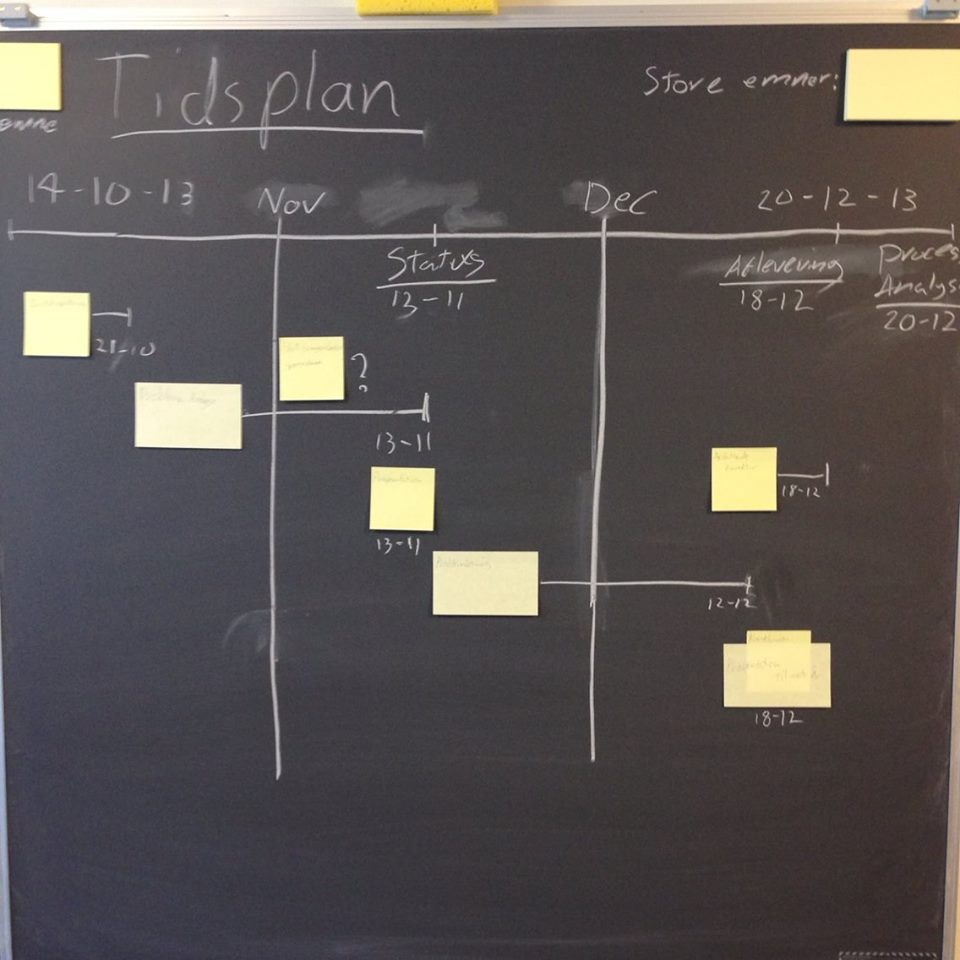
\includegraphics[width=3in]{tidsplan.jpg}
    \caption{Første udkast til tidsplan}
\end{figure}
\clearpage
I arbejdet med vores projekt og rapportstrukturering, har vi anvendt den orange model fra PV.

\begin{figure}[h]
    \centering  
    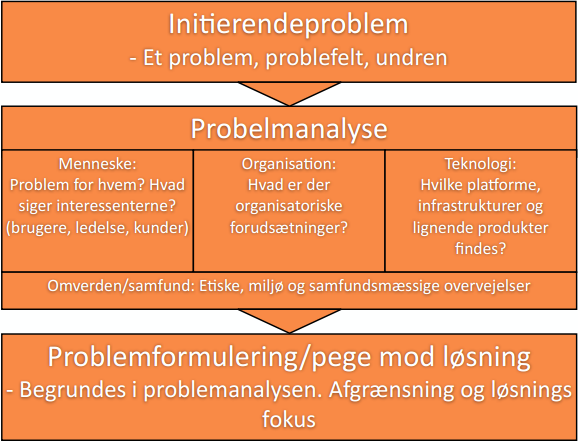
\includegraphics[width=3in]{orange.png}
    \caption{Problem-baseret projektarbejde}
\end{figure}
Modellen har vi brugt til at strukturere vores arbejde; til at sørge for at vi kom omkring det hele og til at sørge for at rapporten har den korrekte opdeling, sådan at problemanalysen forbliver det og ikke bliver til et teoriafsnit.
Ligeledes har vi også brugt studieordningen, i samarbejde med vore vejledere, til at sørge for at projektet opfylder de krav der bliver stillet i forhold til viden, færdigheder og kompetencer.
\clearpage
En del af dette er at dokumentere arbejdsprocessen, hvilket vi har forsøgt at gøre vha. billeder:
\begin{figure}[ht!]
    \centering
    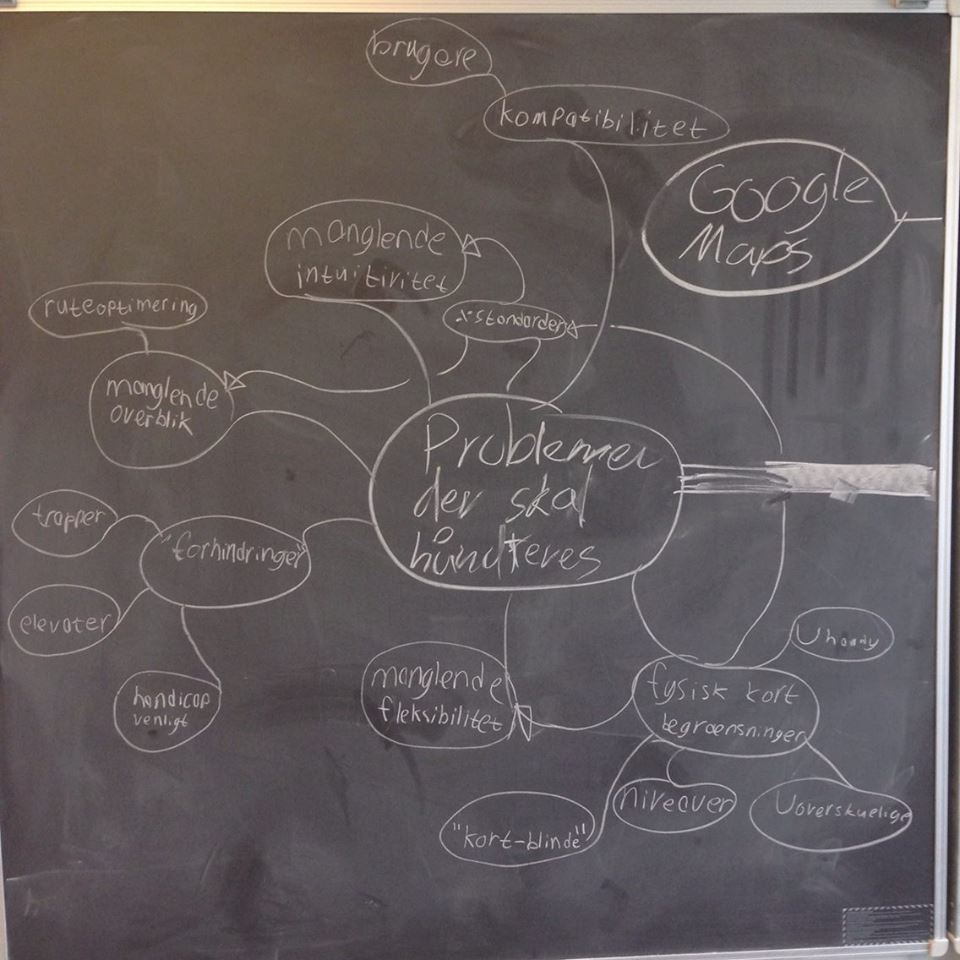
\includegraphics[width=3in]{tavle1.jpg}
\end{figure}
\begin{figure}[ht!]
    \centering
    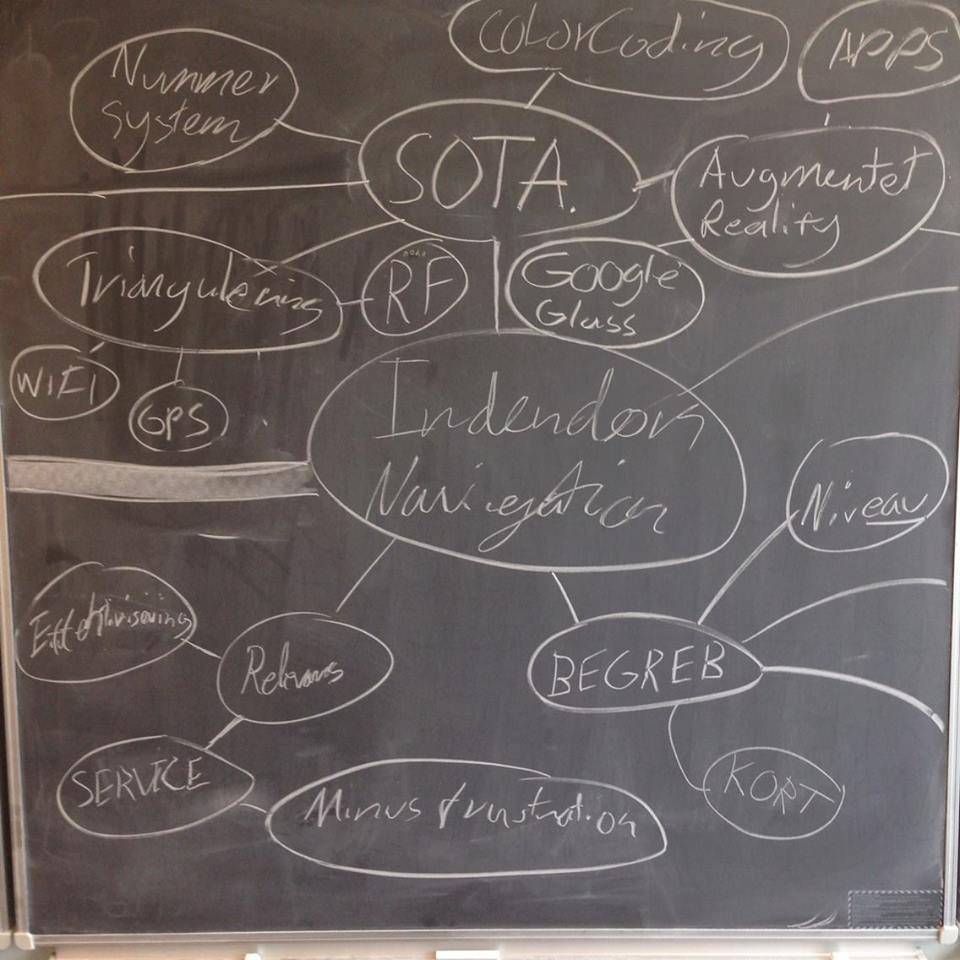
\includegraphics[width=3in]{billede2.jpg}
\end{figure}
\clearpage
\begin{figure}[ht!]
    \centering
    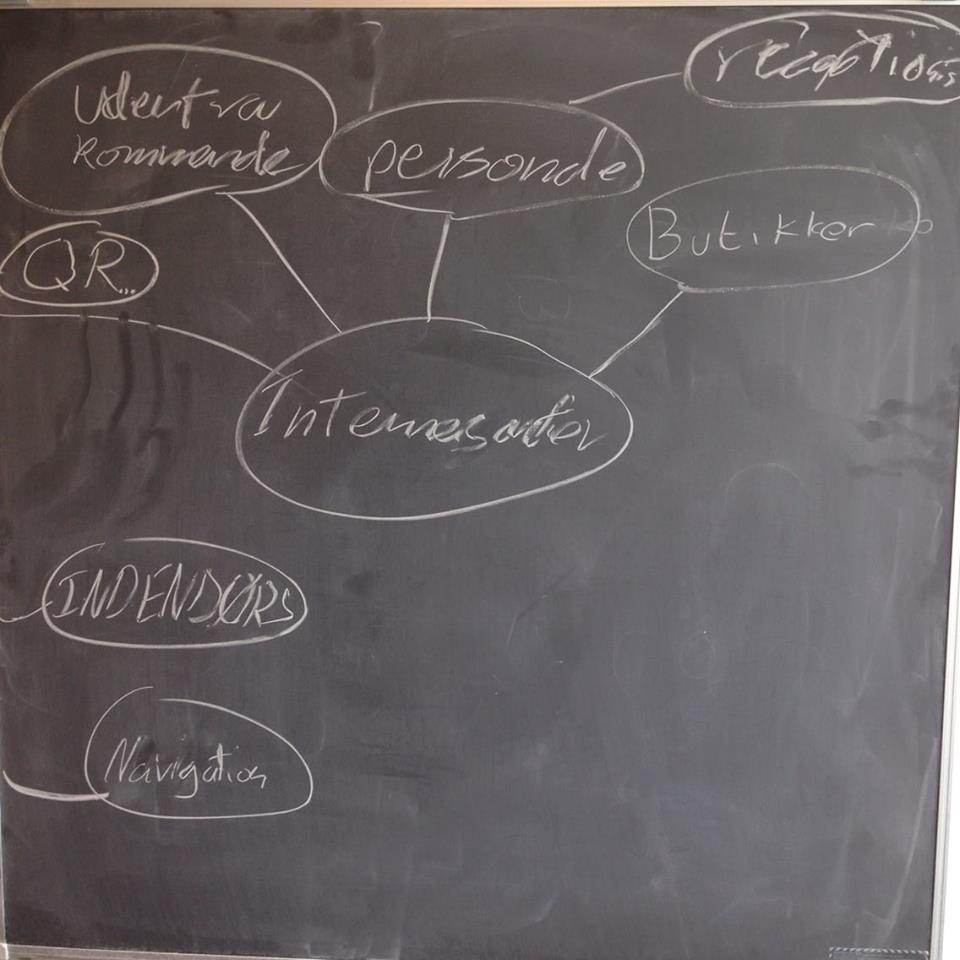
\includegraphics[width=3in]{billede3.jpg}
    \caption{Mindmap over brainstorm lavet ud fra vor initierende problem}
\end{figure}
Vores efterfølgende arbejdsproces bestod i flere iterationer af gruppediskussion efterfulgt af informationssøgning og tilhørende skrivearbejde. Gruppediskussionerne bestod af en ligelig fordeling mellem diskussioner omkring projektets videre forløb, og af forelæsninger hvor gruppens medlemmer fortalte og forklarede hvad de havde fundet ud af.\\
Undervejs i arbejdsprocessen når gruppen gik i stå, håndterede vi dette ved at bytte emner, sådan at vi fik et frisk sæt øjne på emnet. Dette har hjulpet os med at holde retningen på projektet, da vi på et tidspunkt var på vej ud af en tangent med for meget teori.

\end{document}